\section{Введение}
В данной работе проводится многократное прямое измерение периода следования импульсов с помощью электронного частотомера Ч3–32, статистическая обработка полученных результатов и анализ погрешностей.

\subsection{Цель работы}

Целью данной работы является освоение методики многократного прямого измерения физической величины (периода следования импульсов) и выполнение простейшей статистической обработки серии результатов наблюдений для определения наилучшей оценки измеряемой величины и её погрешности.

\subsection{Решаемые задачи}
Для достижения поставленной цели необходимо решить следующие задачи:
\begin{enumerate}
    \item Ознакомиться с устройством и правилами работы с генератором Г5-2А и электронным частотомером Ч3-32.
    \item Собрать установку по блок-схеме (рис.~\ref{fig:setup}) и под руководством преподавателя провести измерения периода следования импульсов на грубой и точной шкалах прибора.
    \item Выполнить многократные наблюдения (10 – на грубой шкале, не менее 50 – на точной шкале).
    \item Провести статистическую обработку результатов: вычислить среднее арифметическое, дисперсию, стандартное отклонение, стандартное отклонение среднего, построить гистограмму распределения и график зависимости результатов от времени.
    \item Оценить погрешность измерения, сравнить её с приборной погрешностью и представить окончательный результат в стандартной форме.
\end{enumerate}

\section{Основная часть}

\subsection{Теоретическая часть}
Среднее арифметическое результатов отдельных наблюдений:
\begin{equation}
    \overline{x} = \frac{1}{n}\sum_{i=1}^{n} x_i .
    \label{eq:mean}
\end{equation}

Дисперсия:
\begin{equation}
    \sigma = \sqrt{\frac{1}{n-1}\sum_{i=1}^{n}(x_i - \overline{x})^2} .
    \label{eq:var}
\end{equation}

Относительная и абсолютная погрешности прибора соответственно:
\begin{equation}
    \gamma_{T1} = \pm (\gamma_0 + \frac{T_0}{\overline{x} \cdot 10^n}) \cdot 100\% ,
    \label{eq:gamma}
\end{equation} где $\gamma_0 = 5 \cdot 10^{-7}$ --- погрешность частотного генератора при измерении в течение 1 часа, $T_0$ --- период интегрирования данных равный $10^{-4}$ с для грубой шкалы и $10^{-6}$ с для точной.
\begin{equation}
    \Delta T_{\textit{приб}} = \frac{\gamma_{T1} \cdot \overline{x} }{100\%}.
    \label{eq:device_err}
\end{equation}


\subsection{Эксперимент}
Схема экспериментальной установки приведена на рис.~\ref{fig:setup}. Генератор Г5-2А вырабатывает последовательность трапецеидальных импульсов, параметры которых (амплитуда, длительность, период) задаются преподавателем. Период следования импульсов измеряется универсальным электронным частотомером Ч3-32.

\begin{figure}[ht!]
\centering
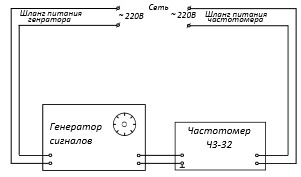
\includegraphics[width=0.8\textwidth]{Sketch}
\caption{Схема установки}
\label{fig:sketch}
\end{figure}



\begin{figure}[ht!]
\centering
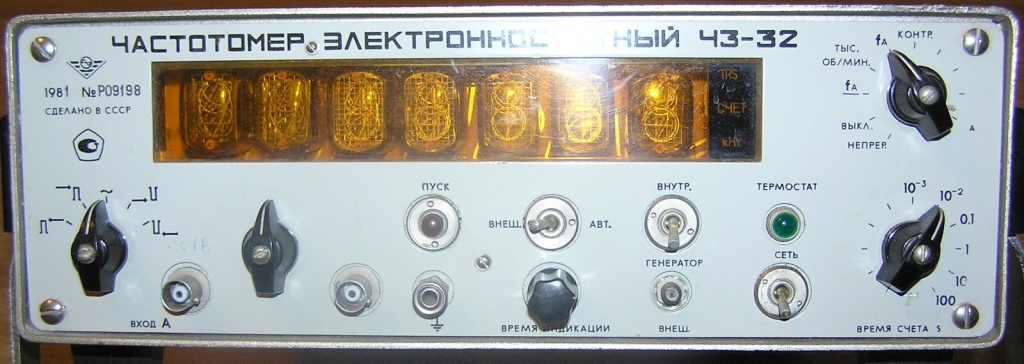
\includegraphics[width=0.8\textwidth]{Device}
\caption{Фотография прибора ЧЗ-32}
\label{fig:device}
\end{figure}

\subsection{Обработка данных и обсуждение результатов}
Первоначально на грубой шкале частотомера (диапазон 0–$10^6$ мс) было выполнено 10 измерений периода следования импульсов. Результаты занесены в табл.~\ref{tab:rough}. Затем на точной шкале (диапазон 0–$10^4$ мс) проведено 50 наблюдений для получения выборки со случайным разбросом (табл.~\ref{tab:exact}).

\begin{table}[ht!]
\centering
\caption{Результаты измерений на грубой шкале}
\label{tab:rough}
\begin{tabular}{|c|c|c|c|}
\hline
№ п.п. & Диапазон шкалы, мс & \(T_i\), мс & \(\Delta T_{\textit{приб}}\), мс \\
\hline
1  &      & 273,8 &  \\
2  &      & 274,0 &  \\
3  &      & 273,8 &  \\
4  &      & 273,8 &  \\
5  & 0 - $10^6$ & 273,6 & 0,1\\
6  &      & 273,7 &  \\
7  &      & 273,1 &  \\
8  &      & 273,3 &  \\
9  &      & 273,1 &  \\
10 &      & 273,4 &  \\
\hline
\end{tabular}
\end{table}

\begin{table}[ht!]
\centering
\caption{Результаты измерений на точной шкале (приведены первые 5 и последние 5 наблюдений)}
\label{tab:exact}
\begin{tabular}{|c|c|c|c|c|}
\hline
№ & Диапазон шкалы, мс & \(T_i\), мс & \(d_i = T_i-\overline{T}\) & \(d_i^2\) \\
\hline
1  & & 274,414 & 0,479 & 0,230  \\
2  & & 274,576 & 0,641 & 0,411  \\
3  & & 274,321 & 0,386 & 0,149 \\
4  & & 274,064 & 0,129 & 0,017  \\
5  & & 274,535 & 0,600 & 0,360  \\
\dots & $0-10^4$ & \dots & \dots & \dots \\
46 & & 273,571 & -0,364 & 0,132  \\
47 & & 273,791 & -0,144 & 0,021  \\
48 & & 273,330 & -0,605 & 0,366  \\
49 & & 273,808 & -0,127 & 0,016 \\
50 & & 273,366 & -0,569 & 0,323 \\
\hline
\end{tabular}
\end{table}

\subsubsection{Анализ временной зависимости}
Для выявления возможного дрейфа измеряемой величины построены графики зависимости результатов наблюдений от порядкового номера (рис.~\ref{fig:rough_drift}, ~\ref{fig:precise_drift}).

\begin{figure}[h!]
    \center{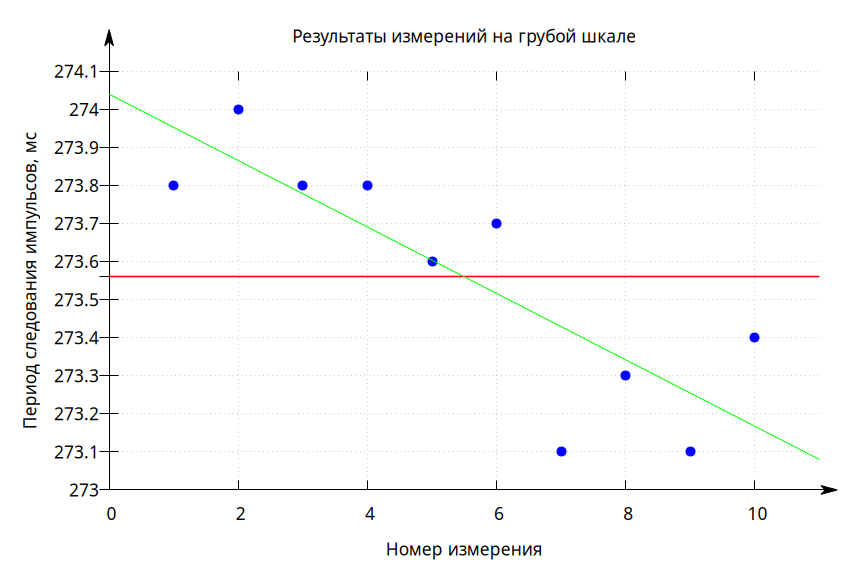
\includegraphics[width=0.8\linewidth]{scatter_rough.png}}
    \caption{График измерений на грубой шкале. Линии: красная -- среднее арифметическое, зелёная -- приближение МНК}
    \label{fig:rough_drift}
\end{figure}

На графике(~\ref{fig:rough_drift}) наблюдается спад значений измеряемой величины со временем. В данном случае этим можно пренебречь, так как количество измерений в данной выборке было не велико.

\begin{figure}[h!]
    \center{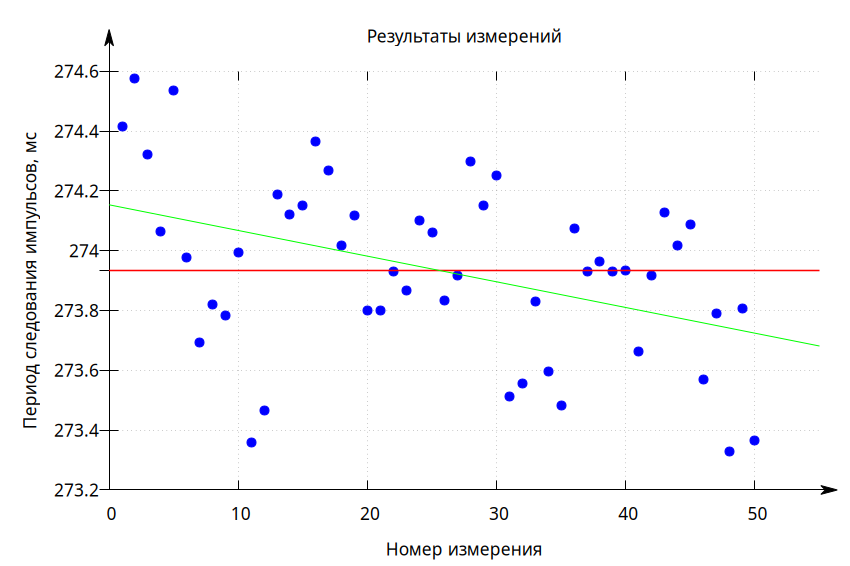
\includegraphics[width=0.8\linewidth]{scatter_precise.png}}
    \caption{График измерений на грубой шкале. Линии: красная -- среднее арифметическое, зелёная -- приближение МНК}
    \label{fig:precise_drift}
\end{figure}
Уравнение, полученное МНК для измерений на точной шкале, имеет вид $y = -0,00858612 \cdot x + 274,154$ (стандартная ошибка наклона $se(\hat{a}) = \pm 0,002676$). Для анализа возможного дрейфа произведём оценку через t-статистику
\begin{equation}
    t = \left| \frac{\hat{a}}{se(\hat{a})}\right|.
\end{equation}
В данном случае $t \approx 3,21$. Для двустороннего критерия при уровне значимости $\alpha = 0,05$ критическое значение распределения Стьюдента с 48 степенями свободы составляет $\approx 2,01$. Так как 3,21 > 2,01, нулевая гипотеза (отсутствие дрейфа, a = 0) отвергается на 5\%-ном уровне значимости. С помощью следующей программы на python получено p-значение равное $\approx 0.0024$.
\begin{lstlisting}[language=Python, label=p-value, caption=Вычисление p-значения]
from scipy.stats import t
t_stat = 0.00858612 / 0.002676
p_value = 2 * t.sf(t_stat, 48)
print(p_value)
\end{lstlisting}
Это означает, что если бы на самом деле дрейф отсутствовал, то вероятность получить столь большое значение $|t|$ (или больше) составила бы всего 0.24\%. Такая малая вероятность указывает на статистически значимый дрейф. Этот момент должен быть учтён при определении доверительного интервала.

\subsubsection{Построение гистограммы}
\paragraph{Грубая шкала}
$x_{min} = 273,1 \space \textit{ мс}$, 
$x_{max} = 274,0 \space \textit{ мс}$.

\begin{table}[ht!]
\centering
\caption{Данные для построения гистограммы}
\label{tab:hist_rough}
\begin{tabular}{|c|c|c|c|}
\hline
№ интервала & Границы интервала, мс & Число попаданий \(\Delta n\) & Доля \(\Delta n / n\) \\
\hline
1  & 273,100 &   &    \\
2  & 273,325 & 3 & 0.3 \\
3  & 273,550 & 1  & 0.1 \\
4  & 273,775 & 2 & 0.2 \\
5  & 274,000 & 4 & 0.4 \\
\hline
Сумма & & 10 & 1.00 \\
\hline
\end{tabular}
\end{table}
\begin{figure}[ht!]
\centering
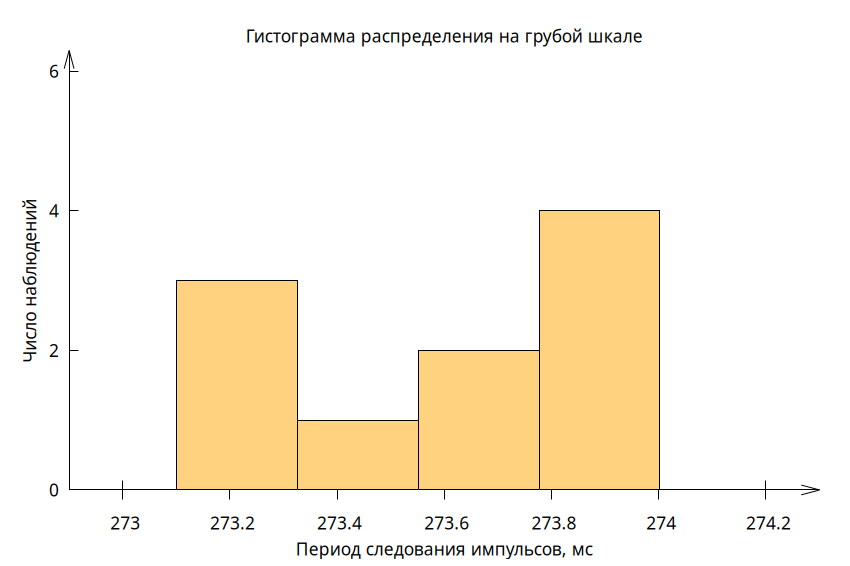
\includegraphics[width=0.8\textwidth]{histogram_rough.png} 
\caption{Гистограмма распределения результатов измерений для грубой шкалы}
\label{fig:hist}
\end{figure}
Беря в расчёт вид гистограммы и количество измерений, построение графика распределения не имеет смысла.

Вычисленные значения по формулам (~\ref{eq:mean})-(~\ref{eq:device_err}): 
$\overline{T} = 273.56 \space \textit{ мс}$,
$\sigma = 0,31693 \space \textit{ мс}$,
$\sigma_{\overline{x}} \approx \Delta T_{\textit{изм}} = 0,1 \space \textit{ мс}$,
$\omega = \Delta T_{\textit{приб}} = 0,1 \space \textit{мс}$.

Итоговый результат измерений:
$T = \overline{T} \pm \sqrt{\Delta T_{\textit{изм}}^2 + (\frac{\omega}{3})^2} = 273,6 \pm 0,1$

\paragraph{Точная шкала}
$x_{min} = 273,330 \space \textit{ мс}$, $x_{max} = 274,576 \space \textit{ мс}$.
Диапазон для построения гистограммы: 273,3 -- 274,6 \textit{мс} будет разбит на 13 промежутков.

\begin{table}[ht!]
\centering
\caption{Данные для построения гистограммы}
\label{tab:hist_precise}
\begin{tabular}{|c|c|c|c|}
\hline
№ интервала & Границы интервала, мс & Число попаданий \(\Delta n\) & Доля \(\Delta n / n\) \\
\hline
1  & 273,3 &   &    \\
2  & 273,4 & 3 & 0.06 \\
3  & 273,5 & 2  & 0.04 \\
4  & 273,6 & 4 & 0.08 \\
5  & 274,7 & 2 & 0.04 \\
6  & 273,8 & 4 & 0,08 \\
7  & 273,9 & 5 & 0.10 \\
8  & 274,0 & 9  & 0.18 \\
9  & 274,1 & 6 & 0.12 \\
10 & 274,2 & 7 & 0.14 \\
11 & 274,3 & 3  & 0.06 \\
12 & 274,5 & 2 & 0.04 \\
13  & 274,6 & 1 & 0.02 \\
13  & 274,6 & 2 & 0.04 \\
\hline
Сумма & & 50 & 1.00 \\
\hline
\end{tabular}
\end{table}


\begin{figure}[ht!]
\centering
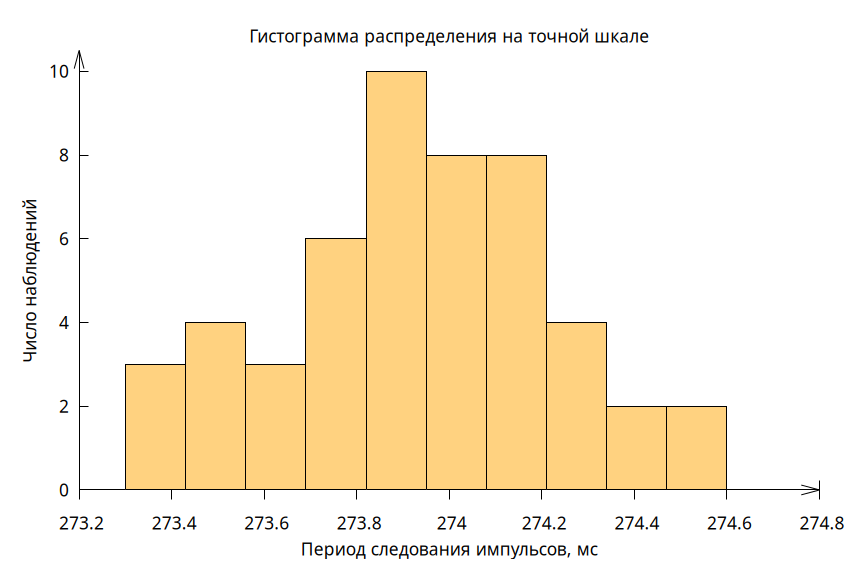
\includegraphics[width=0.8\textwidth]{histogram_precise.png} 
\caption{Гистограмма распределения результатов измерений для точной шкалы}
\label{fig:hist}
\end{figure}

\begin{figure}[ht!]
\centering
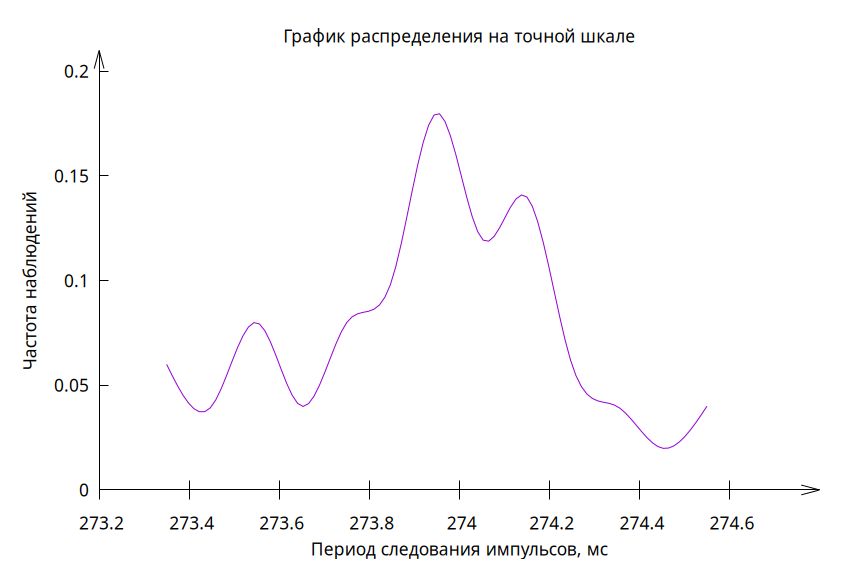
\includegraphics[width=0.8\textwidth]{precise_spline.png} 
\caption{График распределения результатов измерений для точной шкалы}
\label{fig:hist}
\end{figure}
Учитывая отсутствие на графике выраженного пика и распределение далёкое от нормального, проблематично определить по нему дисперсию. Если же это пытаться сделать, взяв ширину графика на 0,6 высоты, то  $2\sigma \approx 0,3$.

Дисперсия рассчитанная по формулам $\sigma = 0,298$

\subsubsection{Статистические расчёты}

Наилучшей оценкой измеряемой величины в некоторый момент времени $t_0$ (например, в середине интервала наблюдений) является значение, предсказанное линейной регрессионной моделью. Считаем, что замеры производились через равные промежутки времени. Тогда для момента $t_0$ точечная оценка: $\hat{y}_0= at_0 + b$.
Погрешность этой оценки для середины интервала вычисляется по формуле:
\begin{equation}
    s_{\hat{y}_0} = \frac{s_{res}}{\sqrt{n}}.
\end{equation}

$$s_{\hat{y}_0} \approx 0,273/\sqrt{50} = 0,0386$$ 
Тогда доверительный интервал с $P = 0,95 \space (t_{0,95;48} \approx 2,01)$: $\Delta y_0 = t \cdot \hat{y}_0 = 0,0776$. Сам же $\hat{y}_0 = y(t_0) \approx 273,940$

Итоговая оценка: $T = 273,940 \pm 0,078$. Приборная погрешность не учтена, так как $\Delta T_{\textit{приб}} \approx 0,00114 \textit{ мс} \ll \Delta T_{\textit{изм}}$

\section{Выводы}
В ходе работы проведены многократные измерения периода следования импульсов на грубой и точной шкалах частотомера Ч3-32. Статистическая обработка показала наличие значимого линейного дрейфа (p < 0.05), поэтому прямое усреднение всех наблюдений дало бы смещённую оценку. Корректный результат получен с помощью линейной регрессии: значение периода в середине интервала наблюдений $T=273.940 \pm 0.078 \textit{ мс}$ с доверительной вероятностью 0.95. Приборная погрешность оказалась пренебрежимо мала по сравнению со случайной.

